\chapter{Selected technologies}
As the core of this work will focus on analysing and benchmarking usage of popular distributed system stacks, it is only fair to begin with introducing the selected components from which the system consist.

This chapter should be treated as a brief introduction into the selected technologies, as very detailed explanations and and implementation details will be provided throughout chapters \ref{chap:system-design} through \ref{chap:perf-scalability}.

\section{Hadoop DFS}
As the system will require the storage of many gigabytes (hundreds) of data the core of the system will be pretty much dominated by writing and reading to / from a datastore that contains all our reference video material.

Hadoop's \ref{hadoop} Distributed File System was designed with such thoughts in mind, and is able to scale an abstract file system over many servers, yet providing tools to make it visible as if it was one file system.

\section{Akka}

\todo{say why akka was selected...}

\chapter{System and design overview}
\label{chap:system-design}

The system, from here to be referred to by the name ,,\textit{Oculus}'', is designed with an asynchronous as well as distributed aproach in mind. In order to achieve high asynchrononisity between obtaining new reference data, and running jobs such as ,,\textit{compare video1 with the reference database}'', the system was split into two primary components: 

\begin{itemize}
  \item \textbf{loader} -- which is responsible for obtaining more and more reference material. It persists and initially processes the videos, as well as any related metadata. In a real system this reference data would be provided by partnering content providers, yet for this 
  \item \textbf{analyser} -- which is responsible for preparing and scheduling job pipelines for execution on top of the Hadoop cluster and reference databases.
\end{itemize}

To further illustrate 

\begin{figure}[hc!]
 \centering
  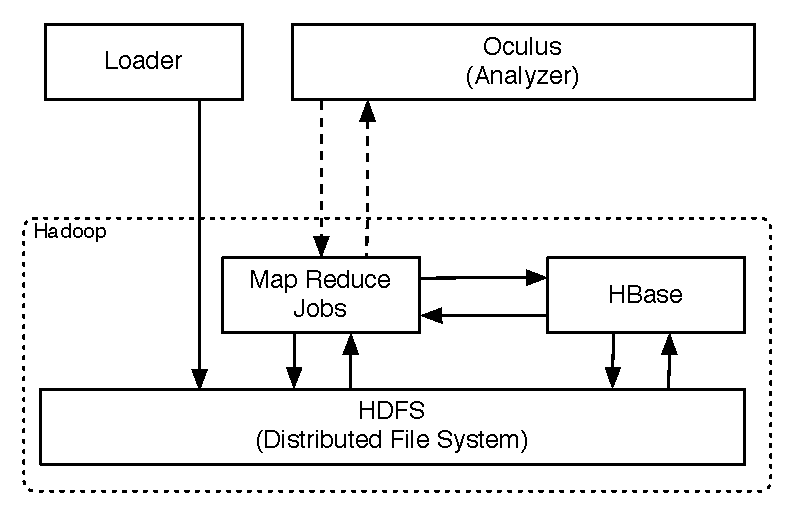
\includegraphics[scale=0.9]{./diagrams/high-level-system.pdf}
  \caption{High level overview of the system's architecture}
  \label{fig:system-overview}
\end{figure}

\section{Loader}
The downloader is responsible for obtaining as much as possible ,,reference data'', by which I mean video material -- from sites such as \textit{youtube.com} or video hosting sites.

It should be also noted that while I refer to this system as ,,the'' downloader, in fact it is composed out of many instances of the same application, sharing the common workload of downloading and converting the input data. The deployment diagram on drawing [12] explains the interactions between the nodes.

\subsection{Work sharing in an actor-based cluster}
The Loader system is implemented following the style of ,,Actor model'' style of concurrency \cite{actor-model}.

This sub-system is implemented the so-called ,,message passing style'', which means that the work requests to the cluster come in as \textit{messages}, and then are \textit{routed} to an \textit{actor}, who performs the work, and then responds with another message -- in other words, all comunication between Actor instances is performed via messages and there is no shared state between them. 
This also applies to Actor instances residing in the same JVM - for the user of an ,,Actor System'', the location (on which phisical node the actor is actually executing) of an actor remains fully transparent - this has huge gains in terms of load balancing the message execution on the cluster - the router decides who will be notified on which message, the listing \ref{lst:akka-router-smallest-inbox} shows a typical workflow using the so-called ,,smallest inbox'' routing strategy \ref{akkaDocs}.

% TODO replace with a drawing with actors
\begin{lstlisting}[caption={smallest-inbox routing algorithm},label={lst:akka-router-smallest-inbox}]
                                                           ---> [inbox1, size = 3] => YoutubeDownloadActor(1)
 YoutubeCrawlerActor -- Msg(url=http://...) --> router ---/
                                                          \     [inbox2, size = 5] => YoutubeDownloadActor(2)
                                                                   
                                  /* because inbox1.size < inbox2.size */ 
\end{lstlisting}

The underlying Actor System is implemented by a project called Akka \cite{akka-docs}, and can be easiest explained as ,,porting Erlang concepts of the Actor Model to the JVM''. I selected the ,,Smallest Inbox'' routing strategy instead of the other widely used ,,Round Robin'' approach in order to guarantee not overloading any Actor with too many requests to download movies (which is a relatively slow process). Thanks to the smallest inbox routing, I can guarantee that if some of the nodes have a faster connection to the Internet, they will get more movie download requests, than nodes located on a slower network.

As mentioned before, the system is fully distributed and \textit{any node can perform any task} submited to the cluster. For example let's take the first step in the processing pipeline in Oculus, which is \verb|Download video from http://www.youtube.com/watch?v=-X9bcrJ3TjY| -- such message will be emited by the \verb|YoutubeCrawlerActor| and sent via a \verb|Router| instance to an \verb|YoutubeDownloadActor| which has the ,,smallest inbox''.


\section{Analyser}
The job runners responsibility is at the core of the systems... \todo{finish describing the analyser}

\subsection{Tackling the ,,small--files problem'' on HDFS}
In this section I will explain the ,,small-files problem'' which would lead to major performance degradation of the Hadoop cluster is left undressed and how it was solved
in the face of having to work with millions of small files -- frames of the analysed movies.

Hadoop uses so called ,,blocks'' as smallest atomic unit that can be used to move data between the cluster.
The default block size is set to \textit{64 megabytes} on most Hadoop distributions (including vanilla Apache Hadoop which this implementation is using).

This also means that if the DFS takes a write of one file (assuming the \textit{replication factor} equals 1) it will use up one block.
By itself this is not worrisome, because other than in traditional (local) file systems such as EXT3 for example, when we store N bytes in a block on HDFS,
the the file system can still use block's unused space. Figure \ref{fig:no-sequence-file} shows the structure of a block storing only one frame of a movie.

\begin{figure}[ch!]
  \centering
  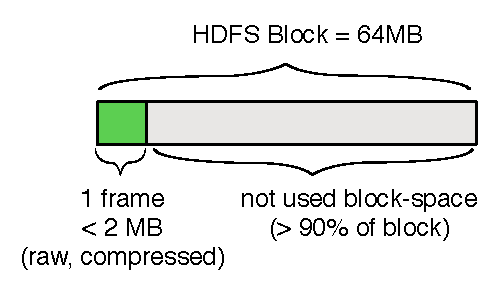
\includegraphics[scale=0.9]{diagrams/no-sequence-file.pdf}
  \caption{When storing a small file in HDFS, it still takes up an entire block. The grey space is not wasted on disk, but causes the \textit{name-node} memory problems.}
  \label{fig:no-sequence-file}
\end{figure}

The problem stemming from writing small files manifests not directly by impacting the used disk space, but in increasing memory usage in the clusters so called \textit{name-node}. The name-node is responsible for acting as a lookup table for locating the blocks in the cluster. Since name-node has to keep 150KB of metadata for each block in the cluster, creating more blocks than we actually need quickly forces the name-node to use so much memory, that it may run into long garbage collection pauses, degrading the entire cluster's performance. To put precise numbers to this -- if we would be able to store 500MB of data in an optimal way, storing them on HDFS would use 8 blocks -- causing the name node to use approximately 1KB of metadata. On the other hand, storing this data in chunks of 2MB (for example by storing each frame of a movie, uncompressed) would use up 250 HDFS blocks, which results in additional 36KB of memory used on the name-node, which is 4.5 times as much (28KB more) as with optimally storing the data! Since we are talking about hundreds of thousands of files, such waste causes a tremendous unneeded load on the name-node.

It should be also noted, that when running map-reduce jobs, Hadoop will by default start one map task for each block it's processing in the given Job. Spinning up a task is an expensive process, so this too is a cause for performance degradation, since having small files causes more \textit{Map tasks} being issued for the same amount of actual data Hadoop will spend more time waiting for tasks to finish starting and collecting data from them than it would have to.

\subsubsection{Sequence Files}
\label{sequence-file}
The solution applied in the implemented system to resolve the small files problem is based on a technique called ,,Sequence Files'', which are a manually controlled layer of abstraction on top of HDFS blocks. There are multiple Sequence file formats accepted by the common utilities that Hadoop provides \cite{hadoop-seq-files} but they all are \textit{binary header-prefixed key-value formats}, as visualised Figure \ref{fig:sequence-file}.


\begin{figure}[ch!]
  \centering
  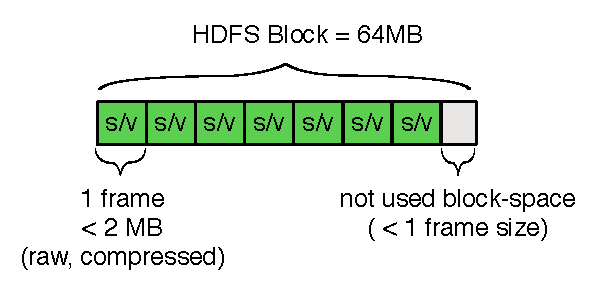
\includegraphics[scale=0.9]{diagrams/sequence-file.pdf}
  \caption{A SequenceFile allows storing of multiple small chunks of data in one HDFS Block.}
  \label{fig:sequence-file}
\end{figure}

Using Sequence Files resolves all previously described problems related to small files on top of HDFS. Files are no longer ,,small'', at least in Hadoop's perception,
since access of frames of a movie is most often bound to access other frames of this movie we don't suffer any drawbacks from such storage format.

Another solution that could have been applied here is the use of HBase and it's key-value design instead of the explicit use of Sequence Files, yet this would not yield much performance nor storage benefits as HBase stores it's Table data in a very similar format as Sequence Files. The one benefit from using HBase in order to avoid the small files problem would have been random access to any frame, not to ,,frames of this movie'', but since I don't have such access patterns and it would complicate the design of the system I decided to use Sequence Files instead.




